\chapter{Umsetzung}
\label{chap:implementation}

Nachdem die Ziele der angestrebten TypeScript-Migration charakterisiert und die Anforderungen an den geplanten Transpiler ausgeführt wurden, soll im Folgenden der Entwurf und die Details der Implementierung umfassend betrachtet werden. In Abschnitt~\ref{sec:js-transpilers} wurden bereits die verbreitetsten Werkzeuge zur Transformation von JavaScript-Quelltexten vorgestellt und verglichen. Auf Basis dieser Gegenüberstellung wurde schließlich Babel~\autocite{BABEL} als Grundlage der vorliegenden Umsetzung des Transpilers von Flow nach TypeScript gewählt.

\section{Software-Architektur}
\label{sec:software-architecture}

Mit der Entscheidung den Übersetzer als Babel-Plugin zu implementieren, ist dessen Grundarchitektur bereits in Teilen festgelegt, da alle Plugins die vorgegebenen Programmschnittstellen von Babel erfüllen müssen. Bevor auf Einzelheiten der Umsetzung näher eingegangen wird, soll zunächst der grundsätzliche konzeptionelle Aufbau der Anwendung skizziert werden. Abbildung~\ref{fig:architecture-overview} verschafft einen Überblick über die verschiedenen Komponenten des Systems und deren Beziehung zueinander.

\begin{figure}[tbp]
  \centering
  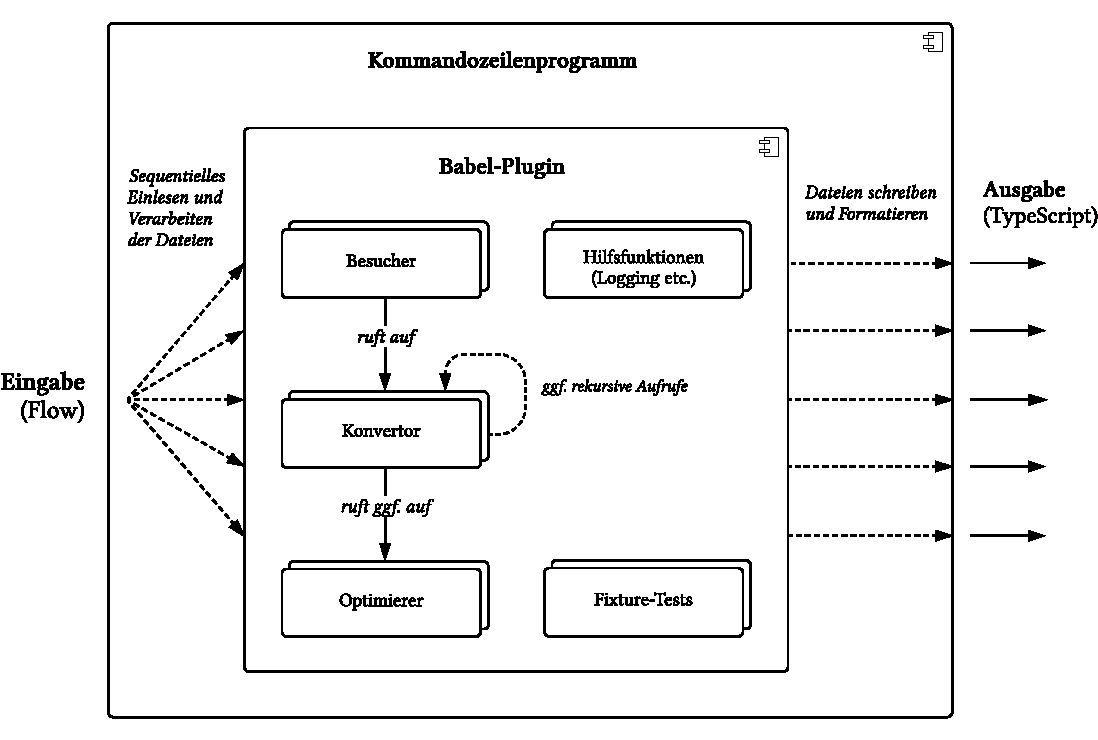
\includegraphics[width=0.92\textwidth]{src/4_Umsetzung/fig/architecture-overview.pdf}
  \caption{Überblick über die Komponenten des Transpilers.}
  \label{fig:architecture-overview}
\end{figure}

Die Architektur gliedert sich in zwei Teile: Ein Kommandozeilenprogramm stellt die Benutzerschnittstelle dar, welche die Eingabe-Verzeichnisse bzw. -Dateien als Argument entgegen nimmt und verschiedene Optionen bereit stellt, um das Verhalten der Übersetzung zu beeinflussen\footnote{Siehe Tabelle~\ref{tab:cli-options}.}. Die zweite Komponente ist das Babel-Plugin, das die Transpilierung des Flow-Codes nach TypeScript realisiert. Das Kommandozeilenprogramm liest sukzessive alle Eingabeverzeichnisse bzw. -dateien ein und startet intern die Übersetzung des Quelltexts durch Babel. Hierfür wird das umgesetzte Plugin geladen und dieses auf die Eingabe angewendet. Danach kann der TypeScript-Code generiert, formatiert und in Dateien oder auf die Standardausgabe geschrieben werden.

Das Plugin setzt sich aus verschiedenen Modulen zusammen: Auf oberster Ebene befinden sich die Besucherfunktionen\footnote{Vgl. Abschnitt~\ref{sec:babel-plugins}.}, welche die eigentliche Programmtransformation realisieren. Diese adressieren alle Pfade des abstrakten Syntaxbaums der Eingabe, die Flow-Syntax darstellen. Bei der Traversierung des Baums durch Babel werden so alle zugehörigen Knoten der Pfade durch Ausführung verschiedener \emph{Konverter} in äquivalentes TypeScript übersetzt. Dabei kann es während der Verarbeitung zu rekursiven Aufrufen weiterer Besucher bzw. Konverter kommen. In einigen Fällen liegen weiterhin Methoden zur Optimierung des Transformationsresultats vor, die nach der Konvertierung gegebenenfalls angewandt werden. Darüber hinaus beinhaltet das Plugin Hilfsfunktionen, um verschiedene Aufgaben wie die Ausgabe von Fehlern und Warnungen umzusetzen. Zuletzt enthält das Plugin eine Vielzahl von Modultests (\textit{Unit tests}), welche die korrekte Funktionalität aller Komponenten überprüfen.

\section{Entwicklungsprozess}

Bevor die Implementierung der Programmtransformation im Detail betrachtet wird, sollen zunächst zwei Aspekte des Entwicklungsprozesses dargelegt werden, die diesen wesentlich unterstützt haben.

\subsection{Testgetriebene Entwicklung}
\label{sec:tdd}

Die korrekte Übersetzung der Flow-Typen nach TypeScript ist wie ausgeführt die wichtigste Anforderung an den Transpiler\footnote{Vgl. Abschnitt \ref{sec:requirement:completeness}.}. Essentiell ist daher die Bereitstellung zuverlässiger Testmechanismen, um Software-Regressionen während der Entwicklungphase frühzeitig festzustellen. Unter Regressionen werden Programmfehler verstanden, die nach bestimmten Ereignissen wie der Implementierung weiterer Funktionen oder Software-Upgrades unvorhergesehen in bereits getesteten Modulen auftreten~\autocite[218]{DOR:SOFTWARE_TEST}. Zur Erfüllung der Anforderung wurde der Ansatz der testgetriebenen Entwicklung\footnote{Engl. \textit{test-driven development} (TDD).} gewählt, um die korrekte Funktionalität und Wechselwirkung aller Bestandteile des Transpilers kontinuierlich zu überprüfen. Die testgetriebene Entwicklung hat ihren Ursprung im Vorgehensmodell \textit{Extreme Programming}~\autocite{JEFFRIES:EXTREME_PROGRAMMING} aus der Software-Entwicklung und sieht im Gegensatz zu klassischen, seriellen Vorgehensweisen wie zum Beispiel dem Wasserfall-Modell vor, dass sämtliche Testfälle einer Funktionalität bereits \emph{vor} dessen Umsetzung geschrieben werden müssen~\autocite{BECK:EXTREME_PROGRAMMING}. Die Vorteile dieser Methodik ist die Gewährleistung einer hohen Testabdeckung~\autocite[90]{BECK:TDD} und die Erzielung einer Implementierung, welche die Anforderungen vollständig erfüllt, sofern die Testfälle sorgfältig konstruiert werden~\autocite[214]{BECK:TDD}. Wenn die Testfälle erst nach der Programmierung angelegt werden, besteht die Gefahr, dass diese lediglich die tatsächlich umgesetzten Funktionen betrachten, jedoch nicht den ursprünglichen, möglicherweise abweichenden Anforderungen gerecht werden.

Der Testaufbau wurde wie folgt konzipiert: Pro Modul wird ein Verzeichnis mit einer Ein\-gabe- und einer Ausgabe-Datei angelegt. Die Eingabe enthält dabei reguläres JavaScript, das mit Flow typisiert wurde, die Ausgabe den äquivalenten, manuell übersetzten TypeScript-Code. In den Dateien können beliebig viele Testfälle einer Kategorie spezifiziert werden, um eine bestimmte Funktionalität des Transpilers zu erproben. Derartige Dateien oder Objekte, die der Initialisierung von Modultests dienen, werden oft als \enquote{\textit{Fixtures}} bezeichnet~\autocite{OLAN:2003}. Durch die bewusste Aufteilung auf zwei unabhängige Dateien kann die inhärente Validität der jeweiligen Quelltexte besser gewährleistet werden, da diese jeweils mittels Flow bzw. TypeScript auf Fehler überprüft werden können. Hierdurch wird vermieden, dass bereits die Testfälle fehlerhaft hinsichtlich der Syntax bzw. der Typisierung erstellt werden. Würden die Quelltexte als Zeichenketten innerhalb der Testumgebung angegeben werden, so wäre eine derartige Prüfung durch das statische Typsystem nicht möglich.

Die Testdurchführung kann nun wie folgt umgesetzt werden: Der Transpiler wird auf die Eingabedatei angewandt und der auf diese Weise generierte TypeScript-Code wird anschließend Zeile für Zeile mit der erwarteten Ausgabe exakt verglichen. Um dies zu erreichen, wurde ein Skript geschrieben, welches das Verzeichnis mit den Modultests einliest, die Transpilierung anstößt und anschließend den zeilenweisen Vergleich durch das Test-Framework \textit{Jest}~\autocite{SOFTWARE:JEST} durchführt. Das angegebene Verzeichnis kann dabei wie in Quelltext~\ref{code:fixture-tests} veranschaulicht beliebig tief verschachtelte Unterverzeichnisse mit Fixture-Dateien enthalten.

\begin{lstlisting}[
  label={code:fixture-tests},
  caption={Fixture-Dateien zum Test der korrekten Transpilierung der Flow-Typen.},
  numbers=none,
  emph={},
]
tests/fixtures
└── types
    ├── any
    │     ├── input.js
    │     └── output.ts
    ├── …
    └── utility
        └── call
            ├── input.js
            └── output.ts
\end{lstlisting}

Während der Entwicklung des Transpilers wurden nach und nach Modultests für alle Funktionen des Programms angelegt. Überprüft wird dabei die korrekte Übersetzung aller Flow-Typen, die Richtigkeit weiterer Optimierungen und die Formatierung der Ausgabe. Weiterhin wurden Tests zur Erprobung des Kommandozeilenprogramms und der allgemeinen Hilfsfunktionen geschrieben. Damit Regression während der fortlaufenden Entwicklung unmittelbar festgestellt werden, werden die Tests nach Einspielung von Änderungen in das Versionverwaltungssystem automatisch ausgeführt (\textit{kontinuierliche Integration}). Insgesamt sind \numberOfTests Testfälle\footnote{Anmerkung: Diese hohe Zahl ist darin begründet, dass größtenteils Fixture-Tests umgesetzt wurden und jeder Vergleich einer nicht-leeren Zeile hierbei als ein Test betrachtet wird.} entstanden und es wurde eine Testabdeckung von 93\% erreicht.
% TODO: check those numbers at the end

\subsection{Statische Typisierung von Babel}

Der gesamte Transpiler, also sowohl das Babel-Plugin, als auch das zugehörige Kommandozeilenprogramm wurden in TypeScript implementiert. Neben den allgemeinen, bereits ausgeführten Vorteilen statischer Typsysteme, ist der primäre Grund hierfür, dass so die durch Babel bereitgestellten Typdeklarationen benutzt werden können. Diese unterstützen die Entwicklungsprozess sehr, weil die Attribute aller Knoten des abstrakten Syntaxbaums von Babel und die Signatur sämtlicher Methoden durch die Typisierung genau spezifiziert sind. Somit kann während der Entwicklung durch den TypeScript-Compiler unmittelbar festgestellt werden, ob fehlerhafte Aufrufe von Bibliotheksfunktionen oder anderweitige Typverletzungen bestehen. Folglich werden inkorrekte Transformationen und Laufzeitfehler reduziert.

Quelltext~\ref{code:babel:static-types} zeigt exemplarisch den Aufbau einer solchen Typdeklaration von Babel anhand des Knotens für ein Typalias in Flow. Dieses besteht aus einem Bezeichner (\code{id}) und einem zugewiesenen Flow-Typ (\code{right}). Der zugewiesene Typ muss dabei ein Element des Vereinigungstyp \code{FlowType} sein, der alle möglichen Typen von Flow umfasst. Darüber hinaus können optional Typparameter des Alias angegeben werden.

\begin{lstlisting}[
  label={code:babel:static-types},
  caption={Externe Typdeklaration des AST-Knotens \textit{TypeAlias} in Babel (Flow).},
  emph={Identifier,TypeParameterDeclaration,null,FlowType},
  keywords={interface,extends},
]
interface TypeAlias extends BaseNode {
  type: "TypeAlias";
  id: Identifier;
  typeParameters: TypeParameterDeclaration | null;
  right: FlowType;
}
\end{lstlisting}

Durch Vergleich der abstrakten Syntaxbäume eines äquivalenten Programmtexts in Flow und TypeScript ist nachvollziehbar, welche TypeScript-Token einem bestimmten Flow-Ausdruck entsprechen. Weil alle Methoden von Babel typisiert sind, ist damit auch bekannt welche Typen als Argument der Funktion, die den bedeutungsgleichen TypeScript-Ausdruck herstellt, erwartet werden. Die Implementierung von Transformationen wird hierdurch erheblich vereinfacht, da so lediglich die Attribute des ursprünglichen Knotens richtig auf den Typ des jeweiligen Funktionsparameters abgebildet werden müssen. Es hat sich während der Entwicklung gezeigt, dass eine derartige Einschränkung durch die Typisierung sehr hilfreich ist: Wenn keine Typfehler mehr vorliegen, ist die Transformation des Flow-Typs nach TypeScript erfahrungsgemäß mit hoher Wahrscheinlichkeit korrekt.

\section{Implementierung als Babel-Plugin}

Nachfolgend soll nun der Aufbau und die konkrete Umsetzung des Babel-Plugins, das die Übersetzung der Flow-Typen nach TypeScript realisiert, erläutert werden.

\subsection{Überblick über Ablauf der Transpilierung}

Abbildung~\ref{fig:activity-diagram-plugin} auf Seite~\pageref{fig:activity-diagram-plugin} veranschaulicht den konzeptionellen Aufbau der Transpilierung innerhalb des Babel-Plugins anhand eines Aktivitätsdiagramms. Aktivitätsdiagramme entstammen der Modellierungssprache \textit{Unified Modeling Language} (UML)~\autocite{OMG:UML} und veranschaulichen die Arbeitsweise von Prozessen innerhalb eines Software-Systems. Zu Beginn wird das Plugin wie im Grundlagenteil in Quelltext~\ref{code:babel-plugin-definition} bereits exemplarisch gezeigt initialisiert, das heißt es wird eine Abbildung der Flow-Knotentypen des abstrakten Syntaxbaums auf Besucher"=Funktionen definiert. Diese realisieren die Transformation aller Flow-Typannotationen in entsprechende TypeScript-Syntax.
Weiterhin werden die Abhängigkeiten des Plugins spezifiziert. Dabei handelt es sich um weitere vorgegebene Babel-Plugins, die benötigt werden, um die Syntax von Flow, JSX und vorläufiger ECMAScript-Erweiterungen einlesen zu können\footnote{Vgl. Anforderung \ref{sec:requirement:syntax}.}. Auf Grundlage der konkreten Anforderungen bei TeamShirts wurden externe Plugins für folgende experimentellen Erweiterungen aktiviert:

\begin{itemize}
  \item \textit{Class field declarations for JavaScript}~\autocite{ES_PROPOSAL:CLASS_FIELDS}
  \item \textit{JavaScript decorators}~\autocite{ES_PROPOSAL:DECORATORS}
  \item \textit{Dynamic imports}~\autocite{ES_PROPOSAL:DYNAMIC_IMPORTS}
\end{itemize}

\begin{figure}[p]
  \centering
  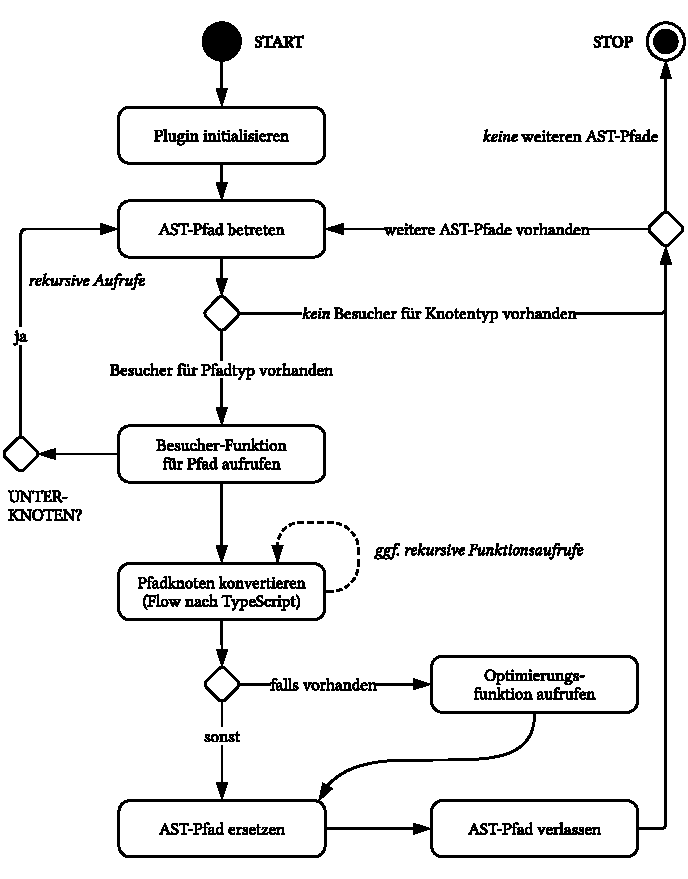
\includegraphics[width=0.85\textwidth]{src/4_Umsetzung/fig/activity-diagram-plugin.pdf}
  \caption{Aktivitätsdiagramm des Transpilers (Babel-Plugin).}
  \label{fig:activity-diagram-plugin}
\end{figure}

Nach der Initialisierung beginnt die rekursive Traversierung des abstrakten Syntaxbaums der Eingabe, um diese umzuformen. Die Datenstruktur des Syntaxbaums wird von Babel durch Parsen des Flow-Programms aufgebaut. Jeder Knoten des Baums wird dabei zunächst \enquote{betreten} und daraufhin wieder \enquote{verlassen}~\autocite{BABEL:HANDBOOK}. Knoten werden verlassen, wenn bei der Beschreitung eines Pfads ein Blatt des Baums erreicht wird und die Traversierung daraufhin auf der höherliegenden Ebene fortgesetzt wird.

Sofern eine Besucherfunktion für den aktuellen Knotentyp existiert, wird diese mit dem zugehörigen Pfad als Argument aufgerufen. Ansonsten wird das nächste Element des Syntaxbaums betreten bzw. die Transpilierung beendet, falls keine weiteren Knoten bestehen. Wenn innerhalb der Besucherfunktion festgestellt wird, dass Kindknoten vorliegen, so wird deren Pfad rekursiv beschritten. Andernfalls wird der Konverter für diesen speziellen Knotentyp ausgeführt, sodass der momentane Pfad anschließend mit dem auf diese Weise berechneten TypeScript-Gegenstück ersetzt werden kann. Gleichzeitig werden für einige Knotenarten Optimierungsfunktionen aufgerufen. Diese korrigieren beispielsweise fehlerhaft verwendete Typen und sind auf die Gegebenheiten der konkreten JavaScript-Projekte abgestimmt. Da viele der Typannotationen von Flow durch mehrere Typen zusammengesetzt werden (zum Beispiel \type{Union type}, \type{Intersection type}, usw.), werden diese Ausdrücke durch mehrere, rekursive Aufrufe von Konvertern umgeformt. Zuletzt wird der momentane Pfad verlassen und die Prozedur beginnt von neuem, sofern weitere Elemente im abstrakten Syntaxbaum vorliegen. Sobald das gesamte Programm und damit sämtliche Flow-Typen übersetzt wurden, kann die TypeScript-Ausgabe mittels des Codegenerators von Babel~\autocite{BABEL:GENERATOR} erzeugt werden.

\subsection{Transpilierung der Flow-Typen}
\label{sec:flow-transpilation}

Im Folgenden soll nun genauer auf den Kern des Transpilers, die Konverterfunktionen, eingegangen werden. Diese realisieren die Übersetzung der einzelnen Flow-Typen nach TypeScript. Aufgrund der großen Zahl von Typen kann nicht die vollständige Umsetzung aller Transformationen und sämtlicher Grenzfälle ausführlich dargelegt werden, da dies den Umfang der Arbeit überschreiten würde. Deshalb wird nachfolgend lediglich ein Überblick über alle Übersetzungen gegeben. Jedoch wurden zur Verbesserung der Anschaulichkeit darüber hinaus einige repräsentative Beispiele ausgewählt, anhand derer das Prinzip der Transpilierung detaillierter erläutert wird, indem die zugrunde liegende Implementierung betrachtet wird. Die genaue Umsetzung aller Transformationen und die Behandlung der Spezialfälle kann mittels des veröffentlichten Quelltexts des Transpilers~\autocite{REFLOW_GITHUB} nachvollzogen werden.

\subsubsection{Transpilierung der Basistypen}

Die Mehrheit der in Tabelle~\ref{tab:flow-base-types} vorgestellten Basistypen von Flow kann innerhalb des Plugins simpel übersetzt werden, da der entsprechende Typ in TypeScript die gleiche Syntax besitzt oder sich lediglich das Schlüsselwort unterscheidet. Von den 30 Basistypen können 18 dieser einfachen Kategorie zugeordnet werden. Die verbleibenden zwölf Typen erfordern komplexere Knotentransformationen, um die Annotationen in entsprechende TypeScript-Ausdrücke umzuwandeln.

\vspace{-0.5\baselineskip}
\paragraph{Simple Übersetzungen}

Tabelle~\ref{tab:transformation-base-types-simple} listet die 18 Flow-Typen auf, die simpel übersetzt werden können und zeigt beispielhaft deren Entsprechung in TypeScript. Abgesehen von den zwei kursiv hervorgehobenen Zeilen ist die Syntax in TypeScript identisch mit der ursprünglichen Notation der Typen in Flow. Dennoch müssen auch diese Elemente des abstrakten Syntaxbaums während der Transpilierung in ihr korrektes Gegenstück umgewandelt werden, da eine Kombination von Flow- und TypeScript-Knoten innerhalb des abstrakten Syntaxbaums gemäß der Spezifikation~\autocite{BABEL:PARSER_SPEC} von Babel verboten ist. Diese Einschränkung wird zur Laufzeit durch Babel mit Hilfe der Bibliothek \code{@babel/types}~\autocite{BABEL:TYPES} sicher gestellt. Aufgrund der Verwendung von TypeScript und der gegebenen Typisierung von Babel werden Typfehler dieser Art aber ohnehin bereits vor Ausführung des Transpilers statisch erkannt.

% \medbreak
\begin{table}[tbh]
  \footnotesize
  \begin{tabu} to \textwidth {@{}lCCX@{}}
    \midrule
    \libertineSB{Basistyp}  & \libertineSB{Flow}            & \libertineSB{TypeScript}         & {} \\
    \midrule
    Any type                & any                           & any                              & {} \\
    Array type              & Array<number>                 & Array<number>                    & {} \\
    Array type (shorthand)  & number[]                      & number[]                         & {} \\
    Boolean literal type    & true                          & true                             & {} \\
    Boolean type            & boolean                       & boolean                          & {} \\
    \textit{Empty type}     & empty                         & never                            & {} \\
    Intersection type       & type Intersection = T1 \& T2  & type Intersection = T1 \& T2     & {} \\
    \textit{Mixed type}     & mixed                         & unknown                          & {} \\
    Null literal type       & null                          & null                             & {} \\
    Number literal type     & 42                            & 42                               & {} \\
    Number type             & number                        & number                           & {} \\
    String literal type     & \str{literal}                 & \str{literal}                    &  {} \\
    String type             & string                        & string                           & {} \\
    This type               & this                          & this                             & {} \\
    Tuple type              & {[}Date, number{]}            & {[}Date, number{]}               & {} \\
    Type alias              & type Type = <FlowType>        & type Type = <TypeScriptType>     & {} \\
    Union type              & number | null                 & number | null                    & {} \\
    Void type               & void                          & void                             & {} \\
    \midrule
  \end{tabu}
  \caption{Übersicht über simple Transformationen der Basistypen von Flow.}
  \label{tab:transformation-base-types-simple}
\end{table}



\begin{lstlisting}[
  % float,
  % floatplacement=htb,
  label={code:example-simple},
  caption={Beispiel für die Übersetzung simpler Flow-Typen.}
]
// @flow                             // TypeScript
type Alias = mixed;                  type Alias = unknown;
\end{lstlisting}

Nachfolgend soll das grundsätzliche Vorgehen bei der Implementierung der Typ"=Transformationen anhand des Ablaufs einer solchen einfachen Übersetzung erläutert werden. Quelltext~\ref{code:example-simple} zeigt links das mit Flow typisierte Ursprungsprogramm und rechts den äquivalenten TypeScript-Code. In der zweiten Zeile wird dabei ein Typalias definiert, welcher auf den Typ \code{mixed} verweist. Wie Tabelle~\ref{tab:transformation-base-types-simple} angibt, ist der korrespondierende TypeScript-Typ \code{unknown}. Um die notwendigen Schritte einer entsprechenden Transformation zu erkennen, ist es hilfreich die abstrakten Syntaxbäume des ursprünglichen und des angestrebten Quelltexts zu vergleichen. Die jeweiligen Syntaxbäume werden in Abbildung~\ref{ast:example-simple} für Flow (links) und TypeScript (rechts) dargestellt\footnote{Anmerkung: Zur Vereinfachung der Nachvollziehbarkeit werden nur wesentliche Teile des Syntaxbaums gezeigt. Tatsächlich besitzen alle Knoten weitere Attribute, die hier jedoch irrelevant sind.}. In den Knoten des Baums steht dabei der Typ des eingelesenen Tokens, die Kanten repräsentieren dessen Attribute. Konkrete Werte wie beispielsweise der Name von Bezeichnern, werden in Anführungszeichen abgedruckt.

\bigbreak
\begin{figure}[htb]
  \centering
  \footnotesize
  \ttfamily
  \begin{subfigure}{.5\textwidth}
    \centering
    \begin{forest}
      for tree = {l=1.6cm, s sep=0.5cm}
      [Program
        [TypeAlias, edge label={node[edge]{body}}
          [Identifier, edge label={node[edge]{id}}
            [\enquote{Alias}, edge label={node[edge]{name}}]
          ]
          [MixedTypeAnnotation, edge label={node[edge]{right}}]
        ]
      ]
    \end{forest}
  \end{subfigure}%
  \begin{subfigure}{0.5\textwidth}
      \centering
      \begin{forest}
        for tree = {l=1.6cm, s sep=1cm}
        [Program
          [TSTypeAliasDeclaration, edge label={node[edge]{body}}
            [Identifier, edge label={node[edge]{id}}
              [\enquote{Alias}, edge label={node[edge]{name}}]
            ]
            [TSUnknownKeyword, edge label={node[edge]{typeAnnotation}}]
          ]
        ]
      \end{forest}
  \end{subfigure}
  \vspace{0.25cm}
  \caption{Abstrakter Syntaxbaum für die Deklaration eines Typalias in Flow (links) und TypeScript (rechts).}
  \label{ast:example-simple}
\end{figure}

Die zwei Bäume sind sich sehr ähnlich: In der Wurzel der Datenstruktur befindet sich bei allen durch Babel eingelesenen Quelltexten der Knoten \code{Program}. Dessen Kindknoten repräsentiert die Deklaration des Typalias aus der zweiten Zeile des Beispiels. Der Typ dieses AST-Elements ist bei Flow \code{TypeAlias} und bei TypeScript \code{TSTypeAliasDeclaration}. Auf der linken Seite der Anweisung steht dabei der Bezeichner des Alias und auf der rechten Seite der zugewiesene Typ.
Weil im ursprünglichen Code das Alias auf \code{mixed} (\code{MixedTypeAnnotation}) verweist, muss dieser Knoten in TypeScript zu \code{unknown} (\code{TSUnknownKeyword}) übersetzt werden, um einen äquivalenten Ausdruck zu erzeugen. In diesem konkreten Fall sind die zwei notwendigen Transformationschritte damit folgende:

\begin{itemize}
  \item Übersetzung des \code{TypeAlias}-Knotens nach \code{TSTypeAliasDeclaration}
  \item Übersetzung des \code{MixedTypeAnnotation}-Knotens nach \code{TSUnknownKeyword}
\end{itemize}

Der erste Schritt, also die Übersetzung des Typalias, wird durch eine Konverterfunktion realisiert, die innerhalb des Besuchers für \code{TypeAlias}-Knoten aufgerufen wird. Quelltext~\ref{code:convert-type-alias} zeigt deren vereinfachten Aufbau. Hierbei werden in Zeile~4 zunächst die Typparameter durch Aufruf einer weiteren Konvertierungsfunktion in das entsprechende TypeScript-Element transformiert. Daraufhin wird der zugewiesene Typ des Alias übersetzt (Zeile~5). Weil dabei ein \emph{beliebiger} Flow-Typ möglich ist, muss dieser allgemeingültig umgewandelt werden können. Es wurde deshalb eine Funktion \code{convertFlowType} implementiert, die alle Flow-Typen universell auf ihr TypeScript-Gegenstück abbildet.

\begin{lstlisting}[
  % float,
  % floatplacement=htb,
  label={code:convert-type-alias},
  caption={Konvertierungsfunktion für Typaliase.}
]
function convertTypeAlias(
  node: TypeAlias
): TSTypeAliasDeclaration | TSInterfaceDeclaration {
  const tsTypeParameters = convertTypeParameterDeclaration(node.typeParameters);
  const tsTypeAnnotation = convertFlowType(node.right);

  if (isInterfaceTypeAnnotation(node.right))
    return convertInterfaceTypeAlias(node);

  return tsTypeAliasDeclaration(node.id, tsTypeParameters, tsTypeAnnotation);
}
\end{lstlisting}

Babel stellt für sämtliche Knoten des abstrakten Syntaxbaums Methoden bereit, mittels derer diese erzeugt werden können~\autocite{BABEL:TYPES}. Somit kann in Zeile~10 durch Aufruf der Bibliotheksfunktion \code{tsTypeAliasDeclaration} ein TypeScript-Typalias erstellt werden, indem der gleiche Bezeichner sowie die übersetzten Typparameter und der transformierte zugewiesene Typ angegeben werden. In Zeile~7~f. wird außerdem ein Spezialfall behandelt: Während Flow Typaliase für Schnittstellen (\textit{Interfaces}) erlaubt, stellt dies in TypeScript unzulässige Syntax dar. Deshalb werden derartige Typaliase in einen regulären Schnittstellentyp umgeformt.

Der schematische Aufbau der universellen Umwandlungsfunktion \code{convertFlowType} wird in Quelltext~\ref{code:convert-flow-type} gezeigt. In Zeile~10 wird hierbei der zweite Schritt der AST-Transformation, die Übersetzung des \code{mixed}"=Schlüsselworts nach \code{unknown}, umgesetzt. Durch Aufruf der Bibliotheksfunktion \code{tsUnknownKeyword()} wird ein neuer AST-Knoten erzeugt, der das entsprechende Schlüsselwort in TypeScript repräsentiert.
In Zeile~4 wird ein weiteres wichtiges Konzept innerhalb des Transpilers exemplarisch aufgezeigt: Für Knoten des Typs \code{ArrayTypeAnnotation} wird die Umwandlungsfunktion \emph{rekursiv} aufgerufen, da auch hier beliebige Flow-Typen als Argument des Feldtyps angegeben werden können. Wie die Transformation des Typalias bereits zeigt, spielt die Umwandlungsmethode \code{convertFlowType} eine zentrale Rolle innerhalb des Transpilers, da sie in nahezu allen Konvertern aufgerufen wird. Zeile~7 verdeutlicht schließlich, dass nicht alle Knoten so einfach wie der Typ \code{mixed} aus dem Beispiel umgewandelt werden können, da der Aufbau vieler Typen komplexer ist. Die Transformation dieser Knoten wird separat durch jeweilige Konverterfunktionen durchgeführt. Im Folgenden wird die Übersetzung solcher komplizierteren Typen ausgeführt.

\begin{lstlisting}[
  % float,
  % floatplacement=htb,
  label={code:convert-flow-type},
  keywords={function,switch,case,return},
  caption={Universelle Transpilierung beliebiger Flow-Typen nach TypeScript durch zentrale Umwandlungsfunktion.}
]
function convertFlowType(node: FlowType): TSType {
  switch (node.type) {
    case 'ArrayTypeAnnotation':
      return tsArrayType(convertFlowType(node.elementType));
    // …
    case 'InterfaceTypeAnnotation':
      return convertInterfaceTypeAnnotation(node);
    // …
    case 'MixedTypeAnnotation':
      return tsUnknownKeyword();
  }
}
\end{lstlisting}

\vspace{-0.5\baselineskip}
\paragraph{Komplexere Übersetzungen}

Die Übersetzung der zwölf komplexen Flow"=Datentypen wird in Tabelle~\ref{tab:transformation-base-types-complex} exemplarisch gezeigt. Im Gegensatz zu den simplen Transformationen unterscheidet sich die Syntax des Ausgabequelltexts hier zum Teil deutlich und es müssen bei der Transpilierung vermehrt Spezial- und Grenzfälle beachtet werden, um korrekten TypeScript-Code zu erzeugen. Zum Beispiel erlaubt Flow den Typ einer Funktion, die eine Zeichenkette und eine Zahl als Argument entgegen nimmt, wie folgt zu deklarieren:

\begin{lstlisting}[numbers=none,aboveskip=10pt]
type FunctionType = (string, argName: number) => void;
\end{lstlisting}

Während die Benennung der formalen Parameter in Flow optional ist, ist diese in TypeScript verpflichtend. Infolgedessen müssen Parameter während der Übersetzung von Funktionstypen nach TypeScript gegebenenfalls automatisch benannt werden, da andernfalls fehlerhafte Syntax entstünde\footnote{Vgl. Zeile~2 in Tabelle~\ref{tab:transformation-base-types-complex}.}.
Der in der Tabelle kursiv hervorgehobene Typ \type{Opaque type} wird in TypeScript nicht unterstützt~\autocite{TS:GITHUB:NO_OPAQUE_TYPE} und wird deshalb wie gezeigt zu einem regulären Typalias umgeformt.

% \medbreak
% TODO sync with chapter 2, maybe line breaks
\begin{longtabuenv}
\begin{longtabu} to \textwidth {@{}lCCX@{}}
  \captionlistentry{Übersicht über komplexe Transformationen der Basistypen von Flow.} \\
  \midrule
  \libertineSB{Basistyp} & \libertineSB{Flow} & \libertineSB{TypeScript} & {} \\
  \midrule
\endfirsthead
  \midrule
  \libertineSB{Basistyp} & \libertineSB{Flow} & \libertineSB{TypeScript} & {} \\
  \midrule
\endhead
  \midrule
  \caption[]{Übersicht über komplexe Transformationen der Basistypen von Flow.}
\endfoot
  Exact object type          & \{| prop: any |\}                &   \{ prop: any \}                      & {} \\
  Function type              & (string, \{\}) => number         &   (p1: string, p2: \{\}) => number     & {} \\
  Generic type annotation    & let v: <{}FlowType>{}            &   let v: <{}TSType>{}                  & {} \\
  Generics                   & type Generic<{}T: Super> = T     &   type Generic<{}T extends Super> = T  & {} \\
  Interface type             & interface I \{ +prop: number \}  &   interface I \{ readonly: number \}   & {} \\
  Nullable type (Maybe type) & ?number                          &   number | null | undefined            & {} \\
  Object type                & \{ {[}string{]}: number \}       &   \{ {[}key: string{]}: number \}      & {} \\
  \textit{Opaque type}       & opaque type Opaque = number      &   type Opaque = number                 & {} \\
  Type cast expresssion      & (variable: string)               &   (variable as string)                 & {} \\
  Type export                & export type T = number | null    &   export T = number | null             & {} \\
  Type import                & import type T from \str{./types} &   import T from \str{./types}          & {} \\
  Typeof type                & typeof undefined                 &   undefined                            & {}
  \label{tab:transformation-base-types-complex}
\end{longtabu}
\end{longtabuenv}


% \pagebreak
Anhand des Typs \type{Nullable} soll im Folgenden das Vorgehen bei der Transformation eines komplizierteren Knoten erläutert werden\footnote{Anmerkung: Es wurde ein verhältnismäßig unkompliziertes Beispiel ausgewählt, weil die Ausführung anderer deutlich komplexerer Fälle nicht in prägnanter Form dargelegt werden könnte.}. Dieser Typ wird in der Flow-Dokumentation auch als \enquote{\type{Maybe type}} bezeichnet und wird für die Typisierung optionaler, möglicherweise undefinierter Werte verwendet~\autocite{FLOW:MAYBE_TYPES}. Konkret stellt der Typ die Vereinigung aus dem angegebenen Typ, \code{null} und \code{undefined} dar. In TypeScript existiert keine direkte Entsprechung, aber es kann trivial ein äquivalenter Vereinigungstyps angegeben werden. Quelltext~\ref{code:example-complex} zeigt die jeweilige Deklaration eines Typalias in Flow (links) und TypeScript (rechts), das auf diesen Datentyp verweist.

\begin{lstlisting}[
  % float,
  % floatplacement=htb,
  label={code:example-complex},
  caption={Beispiel für die Übersetzung komplexer Flow-Typen.},
  keywords={type},
  emph={number, null, undefined},
]
// @flow                              // TypeScript
type MaybeNumber = ?number;           type MaybeNumber = number | null | undefined;
\end{lstlisting}

Wie zuvor sollen zunächst die abstrakten Syntaxbäume der Ein- und Ausgabe verglichen werden, um die Einzelschritte der Transpilierung aufzuzeigen. Das Typalias ist dabei analog zum vorherigen Beispiel und dient lediglich der Herstellung korrekter Syntax. Entscheidend ist der zugewiesene Typ des Alias im rechten Teilbaum: Bei Flow liegt hier das Element \code{NullableTypeAnnotation} vor, das den Typ für Zahlen (\code{NumberTypeAnnotation}) als Argument erhält. Auf Seite von TypeScript steht dagegen der Knoten des Vereinigungstyps (\code{TSUnionType}). Diesem ist eine Menge von Typen zugeordnet, die den äquivalenten Ausdruck bilden, indem der Zahlentyp mit den Typen für \code{null} und \code{undefined} kombiniert wird.

\bigbreak
\begin{figure}[htb]
  \footnotesize
  \ttfamily
  \begin{minipage}{.5\textwidth}
    \centering
    \vspace{-1.72cm} % vertically align left tree with right one
    \begin{forest}
      for tree = {l=1.6cm, s sep=0.5cm}
      [Program
        [TypeAlias, edge label={node[edge]{body}}
          [Identifier, edge label={node[edge]{id}}
            [\enquote{MaybeNumber}, edge label={node[edge]{name}}]
          ]
          [NullableTypeAnnotation, edge label={node[edge]{right}}
            [NumberTypeAnnotation, edge label={node[edge]{typeAnnotation}}]
          ]
        ]
      ]
    \end{forest}
  \end{minipage}%
  \begin{minipage}{.5\textwidth}
    \centering
    \begin{forest}
      for tree = {l=1.6cm, s sep=1.25cm}
      [Program
        [TSTypeAliasDeclaration, edge label={node[edge]{body}}
          [Identifier, edge label={node[edge]{id}}
            [\enquote{MaybeNumber}, tier=last, edge label={node[edge]{name}}]
          ]
          [TSUnionType, edge label={node[edge]{typeAnnotation}}
            [TSNumberKeyword, tier=last, edge label={node[edge]{types[]}}, for tree={align=center, minimum width=3cm, l=0, s sep=0, inner ysep=0},
              [TSNullKeyword, no edge
                [TSUndefinedKeyword, no edge]
              ]
            ]
          ]
        ]
      ]
    \end{forest}
  \end{minipage}
  \vspace{0.25cm}
  \caption{Abstrakter Syntaxbaum für die Deklaration eines \enquote{Maybe type} in Flow (links) und TypeScript (rechts).}
  \label{ast:example-complex}
\end{figure}

Quelltext~\ref{code:convert-nullable-type} zeigt die entsprechende Implementierung. Zuerst wird in Zeile~2 das Argument des Typs \code{NullableTypeAnnotation} durch Aufruf der bereits gezeigten, zentralen Umwandlungsfunktion von Flow in den korrekten TypeScript-Typ übersetzt. Im vorliegenden Fall wird Flows \code{NumberTypeAnnotation} in das Gegenstück \code{TSNumberKeyword} überführt. Anschließend wird eine Liste aufgebaut, die aus diesem Datentyp und den Typen für \code{null} und \code{undefined} besteht. Zu Beachten sind hierbei zwei Spezialfälle: Einerseits darf der Nullwert nicht doppelt in die Liste aufgenommen werden (Zeile~4~f.), andererseits müssen Funktionstypen in dieser Situationen geklammert werden, um korrekte Syntax herzustellen (Zeile~6). Eine Doppelung träte dann auf, wenn in Flow der Typ \code{?null} verwendet wird. Zuletzt kann der TypeScript-Vereinigungstyp durch Aufruf der entsprechenden Bibliotheksfunktion von Babel mit der Typliste als Argument erzeugt und zurückgeliefert werden.

\begin{lstlisting}[
  label={code:convert-nullable-type},
  caption={Übersetzung eines \type{Maybe types} in äquivalenten Vereinigungstyp in TypeScript.}
]
function convertNullableTypeAnnotation(node: NullableTypeAnnotation): TSUnionType {
  const tsType = convertFlowType(node.typeAnnotation);
  const types = [
    ...(isTSNullKeyword(tsType)
      ? []
      : [isTSFunctionType(tsType) ? tsParenthesizedType(tsType) : tsType]),
    tsNullKeyword(),
    tsUndefinedKeyword(),
  ];

  return tsUnionType(types);
}
\end{lstlisting}

\subsubsection{Transpilierung der Hilfstypen}

Auch die in Abschnitt~\ref{sec:flow:utility-types} eingeführten Hilfstypen von Flow können größtenteils äquivalent nach TypeScript überführt werden. Tabelle~\ref{tab:transformation-utility-types} gibt einen Überblick über alle Übersetzungen. Für einige der Einträge gibt es in TypeScript bedeutungsgleiche Hilfstypen, andere können leicht durch Verwendung von Typoperatoren abgebildet werden.

% \medbreak
\begin{table}[tbh]
  \footnotesize
  \begin{tabu} to \textwidth {@{}lCCX[l]@{}}
    \midrule
    \libertineSB{Hilfstyp}    & \libertineSB{Flow}     & \libertineSB{TypeScript} & \libertineSB{Anmerkung} \\
    \midrule
    Call                         &  \$Call<F, T...>        & ReturnType<F>              & {} \\
    Class                        &  Class<C>               & typeof T                   & {} \\
    Difference                   &  \$Diff<A, B>           & Omit<A, keyof B>           & {} \\
    Element type                 &  \$ElementType<T, K>    & T[k]                       & {} \\
    Exact                        &  \$Exact<O>             & O                          & {} \\
    Existential type             &  *                      & any                        & Verlust von Typinformation! \\
    Keys                         &  \$Keys<O>              & keyof O                    & {} \\
    None maybe type              &  \$NonMaybeType<T>      & NonNullable<T>             & {} \\
    \textit{Object map}          &  \$ObjMap<O, F>         & any                        & nicht implementiert \\
    \textit{Object map with key} &  \$ObjMapi<O, F>        & any                        & nicht implementiert  \\
    Property type                &  \$PropertyType<O, k>   & O[k]                       & {} \\
    Read only                    &  \$ReadOnly<O>          & ReadOnly<O>                & {} \\
    Read only array              &  \$ReadOnlyArray<A>     & ReadonlyArray<A>           & {} \\
    Rest                         &  \$Rest<A, B>           & Omit<A, Union<keyof B>{>}  & {} \\
    Shape                        &  \$Shape<O>             & Partial<O>                 & {} \\
    \textit{Tuple map}           &  \$TupleMap<T, F>       & any                        & nicht implementiert \\
    Values                       &  \$Values<O>            & O[keyof O]                 & {} \\
    \textit{Subtype}             &  \$Subtype<T>           & any                        & obsolet \\
    \textit{Supertype}           &  \$Supertype<T>         & any                        & obsolet \\
    \midrule
  \end{tabu}
  \caption{Übersicht über Transformationen der Hilfstypen von Flow.}
  \label{tab:transformation-utility-types}
\end{table}


Die Transformation der drei Abbildungstypen \type{Object map}, \type{Object map with key} und \type{Tuple map} wurde nicht umgesetzt, weil kein TypeScript-Ausdruck gefunden werden konnte, der diesen exakt entspricht. Deshalb werden diese Typen bei der Transpilierung mit \type{any} ersetzt. Da die JavaScript-Projekte von TeamShirts diese Hilfstypen jedoch ohnehin nicht verwenden, stellt dies kein Hindernis für die Migration im vorliegenden Fall dar. Die zwei Typen \type{Subtype} und \type{Supertype} wurden wie ausgeführt von Flow als veraltet (\textit{deprecated}) markiert und werden deshalb ebenfalls nach \code{any} übersetzt. Auch der \type{Existential type} wurde als überholt gekennzeichnet, da er unsicher ist~\autocite{FLOW:LINT_RULE_REFERENCE}. Weil TypeScript einen derartigen Typ nicht unterstützt, wird auch dieser durch \code{any} ersetzt. Sollten in der Eingabe einer dieser sechs nicht unterstützen Hilfstypen auftreten, so wird während der Verarbeitung durch das Babel-Plugin wie gefordert eine detaillierte Warnung ausgegeben mit der Aufforderung den Ausgabequelltext an dieser Stelle manuell zu korrigieren\footnote{Vgl. Anforderung~\ref{sec:requirement:completeness}.}.

Zu beachten gilt darüber hinaus, dass die Typparameter der Hilfstypen (\code{F}, \code{T}, \code{O} usw.) für beliebige, kompatible Flow-Typen stehen. Deshalb ruft die Implementierung auch hier intern die universelle Konvertierungsfunktion \code{convertFlowType()} auf, um alle Fälle korrekt zu übersetzen.

\subsubsection{Transpilierung der Typdeklarationen}

Da der Transpiler Anspruch auf Vollständigkeit erhebt, müssen auch Typdeklarationen transformiert werden. Tabelle~\ref{tab:transformation-declarations} zeigt exemplarisch die verschiedenen Deklarationen und deren Gegenstück in TypeScript. Die Syntax ist hierbei ähnlich zu den simplen Basistypen oftmals identisch in Flow und TypeScript. Dennoch müssen die zugrunde liegenden Knoten des abstrakten Syntaxbaums übersetzt werden, da die entsprechenden Ausdrücke in TypeScript eigene Knotentypen besitzen. Interessant ist die Deklaration des Standard-Exports eines Moduls\footnote{Siehe \autocite[377]{ECMASCRIPT:2019}.} in der zweiten Zeile. Während Flow hier den Export von Funktionen unterstützt, kann dies nicht unmittelbar in TypeScript abgebildet werden. Deshalb muss die Deklaration umgeformt werden: Der Wert der ursprünglichen Deklaration wird dabei einer neu erstellten Variablen (\code{\_default}) zugewiesen und kann anschließend als Argument des Exports verwendet werden, sodass ein äquivalenter Ausdruck entsteht.

% \medbreak
% TODO: Sync with chapter 2
\begin{longtabuenv}
\begin{longtabu} to \textwidth {@{}lCK@{}}
  \midrule
  \libertineSB{Deklaration} & \libertineSB{Flow} & \libertineSB{TypeScript} \\
  \midrule
\endhead
  \midrule
  \caption[]{Übersicht über Transformationen der Typdeklarationen von Flow.}
\endfoot
  \captionlistentry{Übersicht über Transformationen der Typdeklarationen von Flow.}
  Class       & declare class C \{\}                 & declare class C \{\}                     \\
  Export      & declare export default () => string  & const \_default: () => string;\newline export default \_default; \\
  Function    & declare function f(number): any      & declare function f(p: number): any       \\
  Interface   & declare interface I \{\}             & declare interface I \{\}                 \\
  Module      & declare module \str{esmodule} \{\}   & declare module \str{esmodule} \{\}       \\
  Type alias  & declare type T = number              & declare type T = number                  \\
  Variable    & declare var v: ?string               & declare var v: string | null | undefined
  \label{tab:transformation-declarations}
\end{longtabu}
\end{longtabuenv}


\subsection{Weitere Optimierungen}
\label{sec:optimizations}

Bei der Erprobung des Transpilers mit den zwei JavaScript-Projekten von TeamShirts wurde die Erfahrung gewonnen, dass neben der Transformation der Flow-Typen auch andere Änderungen des Quelltexts nötig sind, um eine Migration zu TypeScript erfolgreich durchzuführen. Zur Reduzierung händischer Nacharbeit, wurden das Plugin um Funktionen erweitert, die diese zusätzlichen Schritte automatisieren.

\subsubsection{Übersetzung von React Typimporten}
\label{sec:react-type-import-mapping}

Die von TeamShirts eingesetzte Bibliothek React stellt ähnlich wie Babel Typdeklarationen sowohl für Flow, als auch für TypeScript bereit. Diese Typen können importiert und anschließend in den eigenen Typannotation verwendet werden. Leider wurden die korrespondierenden React-Typen in den Definitionen für Flow und TypeScript unterschiedlich benannt. Während einer der Typen in Flow beispielsweise \code{Node} heißt, ist dessen Bezeichnung in TypeScript \code{ReactNode}. Würden die Typimporte unverändert übernommen werden, so entstünden in der Ausgabe Typfehler, da der importierte Typ unter TypeScript nicht existiert.

\begin{lstlisting}[
  label={code:react-imports},
  caption={Import und Benutzung des durch die Bibliothek \textit{React} extern definierten Typs \enquote{Node}.}
]
// @flow                                     // TypeScript
import React, { type Node } from 'react';    import React, { ReactNode } from 'react';
type FunctionType = () => Node;              type FunctionType = () => ReactNode;
\end{lstlisting}

Quelltext~\ref{code:react-imports} veranschaulicht wie die Transpilierung richtig durchgeführt werden sollte. Einerseits muss die Syntax des Typimport als solche transformiert werden, andererseits sollten sämtliche React"=Typen korrekt auf ihr Gegenstück in TypeScript übersetzt werden. Dabei müssen auch alle Konstrukte, die diese importierten Typen verwenden entsprechend angepasst werden. Da bekannt ist, welche Typen durch React definiert sind und wie deren Namen in TypeScript ist, konnte eine solche Transformation mittels einer Abbildungstabelle implementiert werden.

\subsubsection{Konvertierung von Klassendekoratoren}
\label{sec:class-decorators}

In den Projekten von TeamShirts werden \textit{Klassendekoratoren} verwendet, um React"=Komponenten um verschiedene Funktionen zu erweitern. Derartige Dekoratoren sind eine vorgeschlagene Spracherweiterung von ECMAScript, die es ermöglichen Klassen oder deren Attribute, unabhängig von der zugrunde liegenden Implementierung, zu modifizieren~\autocite{ES_PROPOSAL:DECORATORS}. Dabei werden Annotationen (\code{@decorator}) in den Quelltext unmittelbar vor der Deklaration der Klasse bzw. deren Attribute eingefügt. Dekoratoren stellen Funktionen höherer Ordnung dar, die den Konstruktor der Klasse als Argument erhalten, diesen gegebenenfalls verändern und daraufhin eine Funktion zurück liefern, die den Konstruktor intern aufruft~\autocite{ES_PROPOSAL:DECORATORS}. Auf diese Weise kann die Instanziierung aller Objekten dieser Klasse beeinflusst werden, indem beispielsweise weitere Methoden vor oder nach Aufruf des Konstruktors ausgeführt werden.

Es wurde bei der praktischen Erprobung des Transpilers festgestellt, dass die Verwendung von Dekoratoren in TypeScript problematisch ist, da dies zu zahlreichen Typfehlern führt und eine korrekte Typisierung aufwändig ist. Deshalb wurde eine \emph{optionale} Funktion in den Transpiler integriert, welche die Klassendekoratoren durch äquivalente, verschachtelte Funktionsaufrufe ersetzt. Es hat sich gezeigt, dass diese hinsichtlich der Typisierung weitaus weniger Schwierigkeiten verursachen. In Quelltext~\ref{code:class-decorators} wird eine derartige Transpilierung veranschaulicht. Die Transformation der Klassendekoratoren kann durch Setzen der Option \enquote{\code{replace-decorators}} des Kommandozeilenprogramms aktiviert werden\footnote{Vgl. Tabelle~\ref{tab:cli-options}.}.

\begin{lstlisting}[
  % float,
  % floatplacement=H,
  label={code:class-decorators},
  caption={Optionale Übersetzung von Klassendekoratoren in verschachtelte Funktionsaufrufe.}
]
// @flow                                        // TypeScript
@d1(arg)
@d2
class C {}                                      class C {}
export default C;                               export default d1(arg)(d2(C));
\end{lstlisting}

\section{Erweiterung als Kommandozeilenprogramm}
\label{sec:cli-program}

Zur Erfüllung der in Abschnitt~\ref{sec:requirement:batch-processing} dargelegten Anforderung, dass der Transpiler in der Lage sein muss gesamte Projektverzeichnisse zu verarbeiten (Stapelverarbeitung), ist die Erweiterung des Transpilers um ein Kommandozeilenprogramm nützlich. Hierdurch können beliebige Dateien und Verzeichnisse eingelesen und deren Übersetzung durch verschiedene Optionen flexibel gesteuert werden. Wie bereits in Abschnitt~\ref{sec:software-architecture} umrissen benutzt die Konsolenanwendung intern das Babel-Plugin, um die Transpilierung der Flow-Quelltexte nach TypeScript durchzuführen. Die Aufgaben des Programms sind damit das Einlesen der Eingabe, die Delegation dieser an das Babel-Plugin, die Formatierung des generierten TypeScript-Codes und schließlich die Ausgabe desselben.
Die Anwendung wurde als ausführbares Node.js-Skript umgesetzt und \textit{Reflow} benannt. Das Werkzeug kann durch das Paketsystem von Node.js installiert werden und anschließend wie folgt aufgerufen werden\footnote{Siehe~\autocite{REFLOW_GITHUB} für detaillierte Installations-Anweisungen.}. Tabelle~\ref{tab:cli-options} auf Seite \pageref{tab:cli-options} listet alle Kommandozeilenoptionen auf und beschreibt deren Zweck.

\begin{lstlisting}[
  label={code:reflow},
  caption={Aufruf des Kommandozeilenprogramms des Transpilers (\textit{Reflow}).},
  numbers=none,
  emph={},
]
reflow [OPTIONEN]… <DATEIEN ODER VERZEICHNISSE…>
Beispiel: reflow --dry-run --include-pattern "**/*.js" src/
\end{lstlisting}

\medbreak
\begin{table}[tbh]
  \small
  \begin{tabu} to \textwidth {@{}lX[l]@{}}
    \midrule
    \libertineSB{Option} & \libertineSB{Beschreibung} \\
    \midrule
    \medskip
    \texttt{-V -{}-version} & Versionsnummer anzeigen. \\
    \medskip
    \texttt{-d -{}-dry-run} & Generierten TypeScript-Code auf Standardausgabe statt in Dateien schreiben (Testlauf).\\
    \medskip
    \texttt{-e -{}-exclude-dirs <pattern ...>} & Kommaseparierte Liste von Verzeichnissen, die von der Transpilierung rekursiv ausgeschlossen werden sollen. \\
    \medskip
    \texttt{-i -{}-include-pattern <pattern>} & Wildcard-Muster (\textit{glob pattern}) für Eingabedateien bei Angabe von Verzeichnissen (Standardwert: \texttt{"**/*.{js,jsx}"}). \\
    \medskip
    \texttt{-r -{}-replace} & Originaldateien (Flow) mit generierten TypeScript-Dateien ersetzen, statt diese beizubehalten. \\
    \medskip
    \texttt{-D -{}-replace-decorators} & Klassendekoratoren durch verschachtelte Funktionsaufrufe ersetzen (vgl. Abschnitt~\ref{sec:class-decorators}). \\
    \medskip
    \texttt{-h -{}-help} & Hilfe anzeigen. \\
    \midrule
  \end{tabu}
  \caption{Optionen des Kommandozeilenprogramms (\textit{Reflow}).}
  \label{tab:cli-options}
\end{table}


\begin{figure}[tbp]
  \centering
  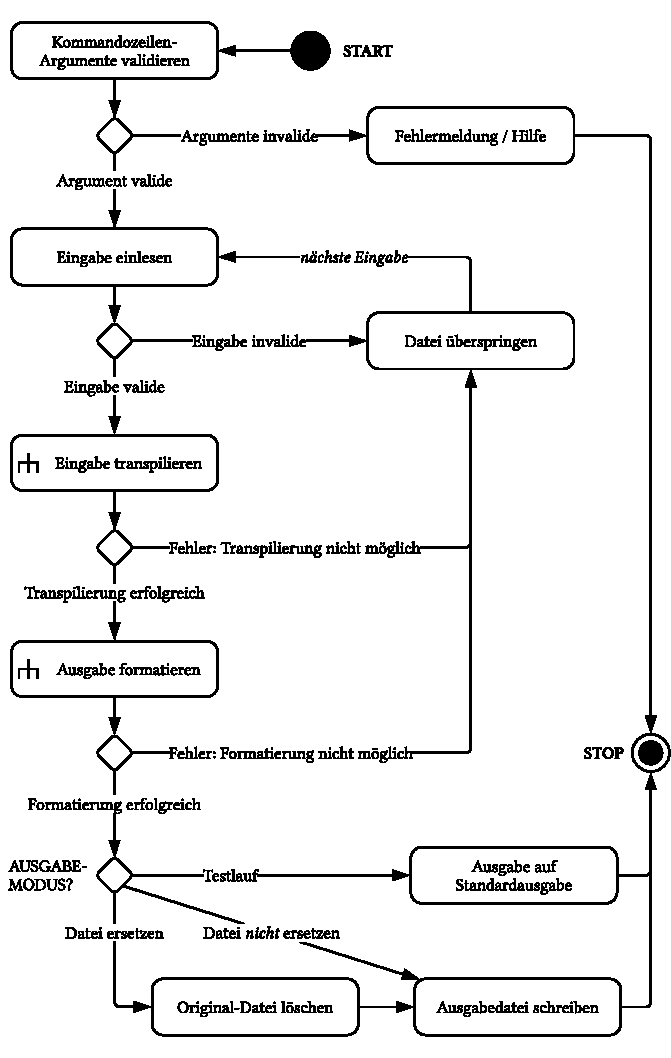
\includegraphics[width=0.85\textwidth]{src/4_Umsetzung/fig/activity-diagram-cli.pdf}
  \caption[Aktivitätsdiagramm des Kommandozeilenprogramms]{Aktivitätsdiagramm des Kommandozeilenprogramms. Vgl. eingebettete Diagramme~\ref{fig:activity-diagram-plugin} \enquote{Eingabe transpilieren} und~\ref{fig:activity-diagram-formatting} \enquote{Ausgabe formatieren}.}
  \label{fig:activity-diagram-cli}
\end{figure}

Abbildung~\ref{fig:activity-diagram-cli} auf Seite~\pageref{fig:activity-diagram-cli} zeigt das Aktivitätsdiagramm des Kommandozeilenprogramms. Als Erstes werden dessen Argumente eingelesen und validiert. Dabei wird überprüft, ob alle Eingabeverzeichnisse bzw. -dateien existieren und ob der Dateityp korrekt ist. Erlaubt sind lediglich JavaScript- und JSX-Dateien. Sofern diese Validierung fehlschlägt, wird die Anwendung mit einer Fehlermeldung beendet. Andernfalls wird daraufhin die Liste aller zu übersetzenden Flow-Dateien erstellt. Falls Verzeichnisse als Argument angegeben worden sind, so werden alle Dateien innerhalb dieser, die dem Wildcard-Muster für Eingabedateien entsprechen, zur Verarbeitungsliste hinzugefügt\footnote{Vgl. Option \code{-{}-include-pattern}.}. Anschließend wird eine Schleife betreten, welche alle Elemente der Liste nach und nach verarbeitet. Da unsinnige Wildcard-Muster durch Benutzereingabe möglich sind, wird erneut überprüft, ob die aktuelle Eingabedatei zulässig ist. Sollte dies nicht der Fall sein, so wird diese übersprungen. Ansonsten wird der Quelltext der Datei durch den Parser von Babel eingelesen und so die Datenstruktur des abstrakten Syntaxbaum des Programms aufgebaut. Daraufhin wird die Transpilierung durch das Babel-Plugin angestoßen. Auch hier kann es zu Laufzeitfehlern kommen, falls beispielsweise Syntaxfehler innerhalb des Eingabequelltexts vorliegen. In diesem Fall wird die aktuelle Datei ebenfalls übersprungen und eine Warnung ausgegeben.

Nachdem die Transpilierung abgeschlossen ist, wird der generierte TypeScript-Code unabhängig von Babel formatiert. Dabei wird eine selbst implementierte Funktion ausgeführt, die eine möglichst originalgetreuen Formatierung der Ausgabe umsetzt. Sollten unerwartete Fehler auftreten wird auch hier die Datei gegebenenfalls übersprungen. Zuletzt kann der generierte TypeScript-Code ausgegeben werden. Dabei gibt es je nach Verwendung der Kommandozeilenoptionen drei Möglichkeiten: Sofern der Parameter \enquote{\code{dry-run}} gesetzt ist, wird das Resultat einfach auf die Standardausgabe geschrieben. Andernfalls werden neue TypeScript-Dateien im Verzeichnis der Eingabedateien erstellt. Falls die Option zum Ersetzen der Originaldateien angegeben wurde, so werden diese zuvor gelöscht.

Da die Verwendung von JSX-Syntax in TypeScript die Dateierweiterung \code{.tsx} vorschreibt~\autocite{TS:HANDBOOK:JSX}, muss sicher gestellt werden, dass die Ausgabedateien die korrekte Endung erhalten. Gleichzeitig müssen globale Typdeklarationen in Dateien mit der Erweiterung \code{.d.ts} geschrieben werden. Zur Bestimmung des korrekten Ausgabedateityps wird deshalb innerhalb des Babel-Plugins während der Transpilierung überprüft, ob JSX-Syntax in der Eingabedatei verwendet wird bzw. ob Typdeklarationen vorliegen. Hierfür werden Besucherfunktionen für diese speziellen AST-Knoten registriert, die eine Lookup-Tabelle aufbauen, welche die Abbildung der Originaldateien auf einen Ausgabetyp darstellt. Das Kommandozeilenprogramm kann diese Information schließlich beim Schreiben der Dateien abfragen und entsprechend reagieren.

\section{Formatierung des Ausgabequelltexts}
\label{sec:formatting}

Ein Aspekt, der sich während der Entwicklung des Transpilers als problematisch herausgestellt hat und deshalb einer gesonderten Betrachtung bedarf, ist die Formatierung des generierten Ausgabecodes. Weil Babel auf Grundlage eines \emph{abstrakten} Syntaxbaums arbeitet, liegt nach der Transformation des Programms keinerlei Information mehr über die ursprüngliche Formatierung des Codes vor. Infolgedessen geht die Einrückung und die Position der Leerzeichen und -zeilen in der TypeScript-Ausgabe verloren. Auch die Position der Kommentare wird nach der Übersetzung nicht präzise beibehalten. Diese werden deshalb von der Übersetzung ausgeschlossen, da sie ohnehin falsch platziert werden. Versuche mit der Option \enquote{\code{retainLines}}~\autocite{BABEL:GENERATOR} des Babel-Codegenerators, welche eine Beibehaltung der Zeilen in der Ausgabe bewirken soll, erzielten leider nicht das gewünschte Ergebnis. Auch nach Setzen dieser Eigenschaft unterscheidet sich das Format des generierten Quelltexts erheblich von der Eingabe.
Da die möglichst originalgetreue Formatierung der Ausgabe aber eine der Anforderungen an den Transpiler ist, wurde eine Formatierungsroutine implementiert, um diese Vorgabe unabhängig von Babel zu erfüllen. Dieses Verfahren wird nach der Transpilierung aller Eingabedateien durch das Kommandozeilenprogramm angestoßen\footnote{Vgl. Abb.~\ref{fig:architecture-overview}.} und soll im Folgenden erläutert werden.

\begin{figure}[htb]
  \centering
  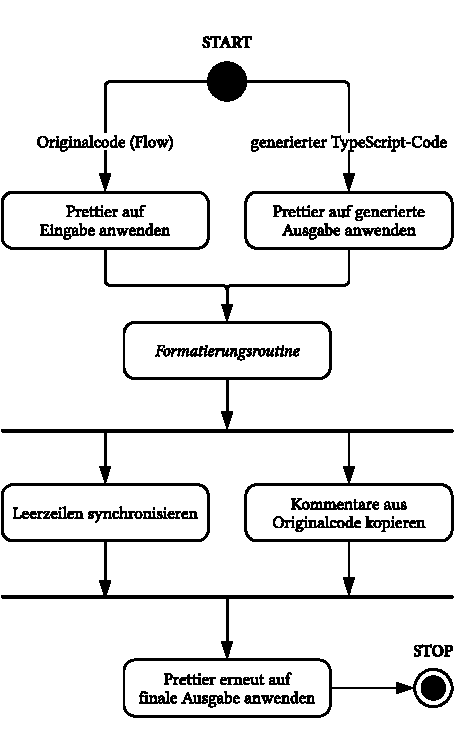
\includegraphics[width=0.55\textwidth]{src/4_Umsetzung/fig/activity-diagram-formatting.pdf}
  \caption[Aktivitätsdiagramm der Formatierung des Ausgabecodes]{Aktivitätsdiagramm der Formatierung des generierten Ausgabecodes.}
  \label{fig:activity-diagram-formatting}
\end{figure}

Der konzeptionellen Aufbau der Formatierungsfunktion wird in Abbildung~\ref{fig:activity-diagram-formatting} dargestellt. Deren Idee ist simpel: Nachdem sowohl die Ein- als auch die Ausgabe in einen vergleichbaren, konsistenten Zustand überführt worden sind, können Leerzeilen und Kommentare aus dem ursprünglichen Quelltext Schritt für Schritt übertragen werden. Konsistent bedeutet, dass die Ausdrücke und Anweisungen in beiden Quelltexten die gleiche Zahl von Zeilen vereinnahmen, also dass diese gleich umgebrochen werden. Diese Voraussetzung muss insbesondere auch für alle Flow-Typen, nach deren Übersetzung nach TypeScript, gelten. Grund für die Herstellung dieser Eigenschaft ist, dass das weitere Verfahren zeilenbasiert arbeitet, um die Originalformatierung in die Ausgabe zu übernehmen.

Zur Herstellung eines solchen Ausgangszustand wird \textit{Prettier}~\autocite{SOFTWARE:PRETTIER} eingesetzt. Prettier ist ein Quelltext-Formatierer, der einen einheitlichen Programmierstil für Sprachen wie JavaScript, TypeScript, HTML und weitere ermöglicht.
Versuche haben gezeigt, dass die Ein- und Ausgabe bei Anwendung von Prettier aufgrund unterschiedlicher Syntax von Flow und TypeScript nicht in allen Situationen übereinstimmend umgebrochen wird. Deshalb wurde das Werkzeugs geringfügig modifiziert, um so eine größere Konsistenz der Ausgabe zu erzielen\footnote{Siehe Anhang~\ref{appendix:prettier}.}. So werden bei Setzen einer neu hinzugefügten Option beispielsweise die Attribute von Objekten immer umgebrochen, um deren Vergleich zu ermöglichen. Prettier bricht diese standardmäßig erst dann um, wenn die eingestellte Druckweite überschritten wird.

Im ersten Schritt der Formatierungsroutine wird diese angepasste Version des Werkzeugs einerseits auf den Originalcode, andererseits auf den generierte TypeScript-Quelltext angewandt. Im Anschluss kann sukzessive über alle Zeilen der Eingabe iteriert werden, um in jedem Schleifendurchlauf zu prüfen, ob eine Leerzeile vorliegt. Gegebenenfalls wird diese an die entsprechende Position in der Ausgabe kopiert. Gleichzeitig werden Block- und Zeilenkommentare im ursprünglichen Flow-Programm gesucht und an die gleiche Stelle in den TypeScript-Code eingefügt. Auf diese Weise werden nach und nach alle Leerzeilen und Kommentare übertragen, sodass die originalgetreue Formatierung hergestellt wird. Schließlich wird Prettier erneut auf die auf diese Weise modifizierte Ausgabe angewandt, um verbleibende Probleme wie beispielsweise doppelte Leerzeilen zu eliminieren.
